\documentclass{article}
\usepackage[utf8]{inputenc}
\usepackage{biblatex}
\usepackage{graphicx}
\usepackage{rotating}
\usepackage{listings}
\usepackage{float}
\usepackage{pdflscape}
\usepackage[english, russian]{babel}
\addbibresource{bib_file.bib}

\title{
    Project in Neural Machine Translation\\
    \large ELEC-E5550 - Statistical Natural Language Processing
}

\author{
  Andrey Sukhobok (795959)\\
  \texttt{andrey.sukhobok@aalto.fi}
  \\[3ex]
  Kosta Stanojević (796026)\\
  \texttt{kosta.stanojevic@aalto.fi}
  \\[3ex]
  Rob Verbeek (766441)\\
  \texttt{rob.verbeek@aalto.fi}
}

\date{April 27, 2020}

\begin{document}

\maketitle

\section*{Abstract}

The current project is completed as a part of Statistical Natural Language Processing course. The aim of the project is exploring modern approaches for Machine Translation using word-vector embeddings.

We used two Deep Learning architectures for this task: Recurrent and Transformer Neural Networks. Two pairs of languages were used to train the networks: English-Dutch and English-Russian. The bilingual evaluation understudy (BLEU) algorithm was used to estimate the quality of the results.

\newpage


\section*{Introduction}

The area of Machine Translation has been actively explored since 1950s. The possible applications of automatic translation systems are endless, since they significantly improve the communication ability between people.

Many statistical models were proposed in the last 20 years. Ideas such as the noisy channel model and alignment methods were relatively effective. In general, the main point is considering the foreign sentence as a noisy version of the original sentence. Using the Bayes Rule, the problem can be decomposed into Language Model and Translation Model. The first one can be an N-gram model or another popular method used for language modelling. For the Translation Model many alignment methods were introduced for different levels of alignment: subwords, words, sentences, etc.

During the last ten years Neural models showed the most promising results. In this project two architectures were tried. Recurrent Neural Networks(RNNs), which are effective for sequence modelling, but which also have a significant disadvantage in speed. The Transformer model was introduced with significant improvements, overcoming the problems of recurrent architectures. The detailed descriptions are provided in the Methods section.

\section*{Data}
We used a dataset from OPUS \cite{opus2018}, based on subtitle data from opensubtitles.org. Opus matched the data, generating one-to-one matches of subtitle data between different languages. This allows us to apply machine translation from one language to the other. Added to that, we are able to train our own word embeddings on this data. For these two purposes, training word embeddings and machine translation, we used slightly different datasets.

\subsection*{Word embeddings}
For the training of word embeddings, we only require single-language corpora, as translations are not taken into account in this training. In addition to aligned subtitle corpora, Opus \cite{opus2018} also provides "raw" subtitle files for each language. Since the data are subtitles, each of the line can be one or more sentences. We used the following datasets for building the word embeddings:

\begin{itemize}
    \item \textbf{English:} 441 450 449 subtitle lines
    \item \textbf{Dutch:} 104 652 076 subtitle lines
    \item \textbf{Russian:} 44 913 765 subtitle lines
\end{itemize}

\subsection*{Machine translation}
For the translation task we use the aligned subtitle data. These are provided to us in two text files, one for each language, with an equal number of (matching) lines:

\begin{itemize}
    \item \textbf{English-Dutch:} 37 200 621 subtitle lines
    \item \textbf{English-Russian:} 25 910 105 subtitle lines
\end{itemize}

\subsection*{Data pre-processing}
For both the embedding data and the translation data we apply the same pre-processing methods. This ensures that the embeddings are trained on the same format of data as the data the translation is performed on, hence making the word embeddings more applicable to the translation task. Because we wanted to keep punctuation, as separate tokens, we use the WordPunctTokenizer of nltk \cite{Loper02nltk:the}. This is a basic tokenizer that splits up sentences into individual words, and in addition splits the punctuation into separate tokens.

We add the <SOS> and <EOS> tokens \textbf{before} we start training the embedding. This way we get a more accurate embedding for these tokens, as well as embedding words at the beginning and the end of the sentence accordingly.

\subsection*{Filtering translation data}
As part of the pre-processing, we added an extra step of filtering to the translation data. Even though the translation set is mostly matched one-to-one, there are some discrepancies. The main ones we found, is that a line of two sentences is only partially translated in the counterpart, and translation is continued in the next line:

\textbf{English:}   I'm not selling any. I'm just curious, that's all.

\textbf{Dutch:} Ik ben alleen nieuwsgierig.\\
\\
The Dutch translation only translates the second part of the English sentence, "I'm just curious", but not the first part. And discrepancies like these are found more often. The were mainly found in pairs where the \textit{lengths between the sentences differed a lot}. Therefore, we created a filter that removes these pairs. For this we use the rule: if the difference in characters is more than 55 percent of the average length of the two sentences, we remove the pair. This rule allows for large difference to still be kept, if the sentences are very long. We do understand that removing part of the data could create some bias, but we made sure that we did not skew the data tremendously, for example by changing the average sentence length of the corpus a lot, as well as not removing too much data.

\selectlanguage{english}
\begin{figure}[H]
    \centering
    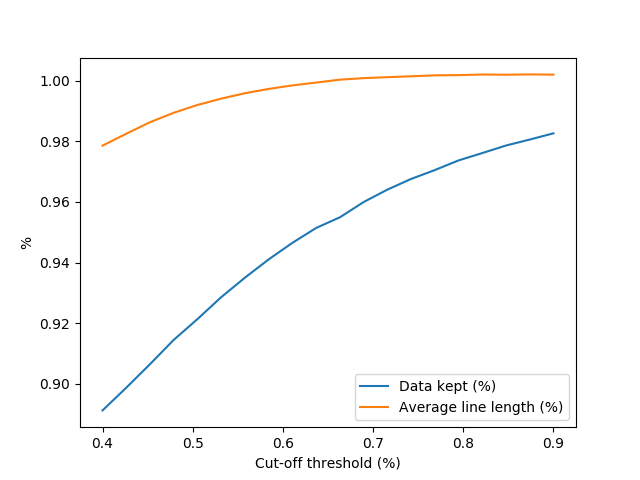
\includegraphics[width=0.9\textwidth]{imgs/cutoff.png}
    \caption{Plot of data statistics for different cut-off thresholds}
    \label{fig:cutoff}
\end{figure}

At a threshold of 0.66 we would exactly preserve the average line length, while keeping approximately 95\% of the data. However, while manually exploring the data, this threshold still left too many discrepancies. After some iterative testing of different thresholds, the value of 0.55 was found to work best, while still preserving 93\% of the data as well as only shrinking the average line length by not even one percent.

\section*{Methods}

In this section we will describe the methods we used for solving the task of machine translation. Firstly, we will describe the architectures of the neural networks. Then, we will discuss the vector models and evaluation scores we used.

\subsection*{Recurrent Neural Network}

Recurrent Neural Networks are a recursive type of neural models that are made to work with sequential data. The recurrence allows the network to memorize previous inputs. This mechanism uses a hidden state. In general, the network has a pair of weight matrices: for input and for the hidden state. And for every subsequent input we provide the hidden state of previous input. This internal memory system allows improvement upon processing of sequences by making use of context of the whole sentence.

However, this architecture has a serious drawback called vanishing and exploding gradient. The problem is connected to the values of derivatives of weights, used in backpropagation, that will significantly decrease or increase the gradients if they are not close to 1. The problem becomes severe when it comes to long sentences. Because of the way RNNs work, where the network is used for every element in the input sequence, they can be imagined as a sequential network with as many layers with shared weights as the length of the input sequence. Thus exceptionally long input sequences essentially produce a sequential network with many layers, which exacerbates the vanishing/exploding gradient problem.

There were several solutions offered to overcome the described issue. The most popular ones are long short-term memory (LSTM) \cite{Schmidhuber1997} and gated recurrent units (GRU) \cite{Cho2014} architectures. For our model, we used the GRU. The main idea of this architecture is introducing the gating mechanism which allow the network to forget the previous information.

For the translation task the Encoder-Decoder architecture is used. We take the input sequence, create a representation of it and then we use this representation as part of the input to the decoder. The decoder predicts the next token of translated sentences starting from the start-of-sentence token using the provided representation and previous tokens.

\subsection*{Transformer Neural Network}

The transformer architecture \cite{Vaswani2017} provided a great improvement for many Natural Language Processing tasks including translation. This model exploits the same Encoder-Decoder architecture as recurrent models. The improvement is that transformer doesn't use recurrent layers, but it uses Linear layers and Multi-Head Attention (MHA) mechanism instead.

The combination of the aforementioned mechanisms has the advantage of taking into account the whole sentence simultaneously, avoiding severe gradient vanishing and using attention. The idea of attention is introducing the Key, Value and Query notations. These are the matrices that represent the words in the sentence. They are multiplied in a way that we train a set of weight matrices to emphasize the corresponding tokens. The end result is that all of the words in the sentence are assigned weights indicating how much the other words influence its' translation.

The scheme of the whole model is provided on the Figure \ref{fig:Transformer}. The picture is copied from the original paper.

\selectlanguage{english}
\begin{figure}
  \centering
  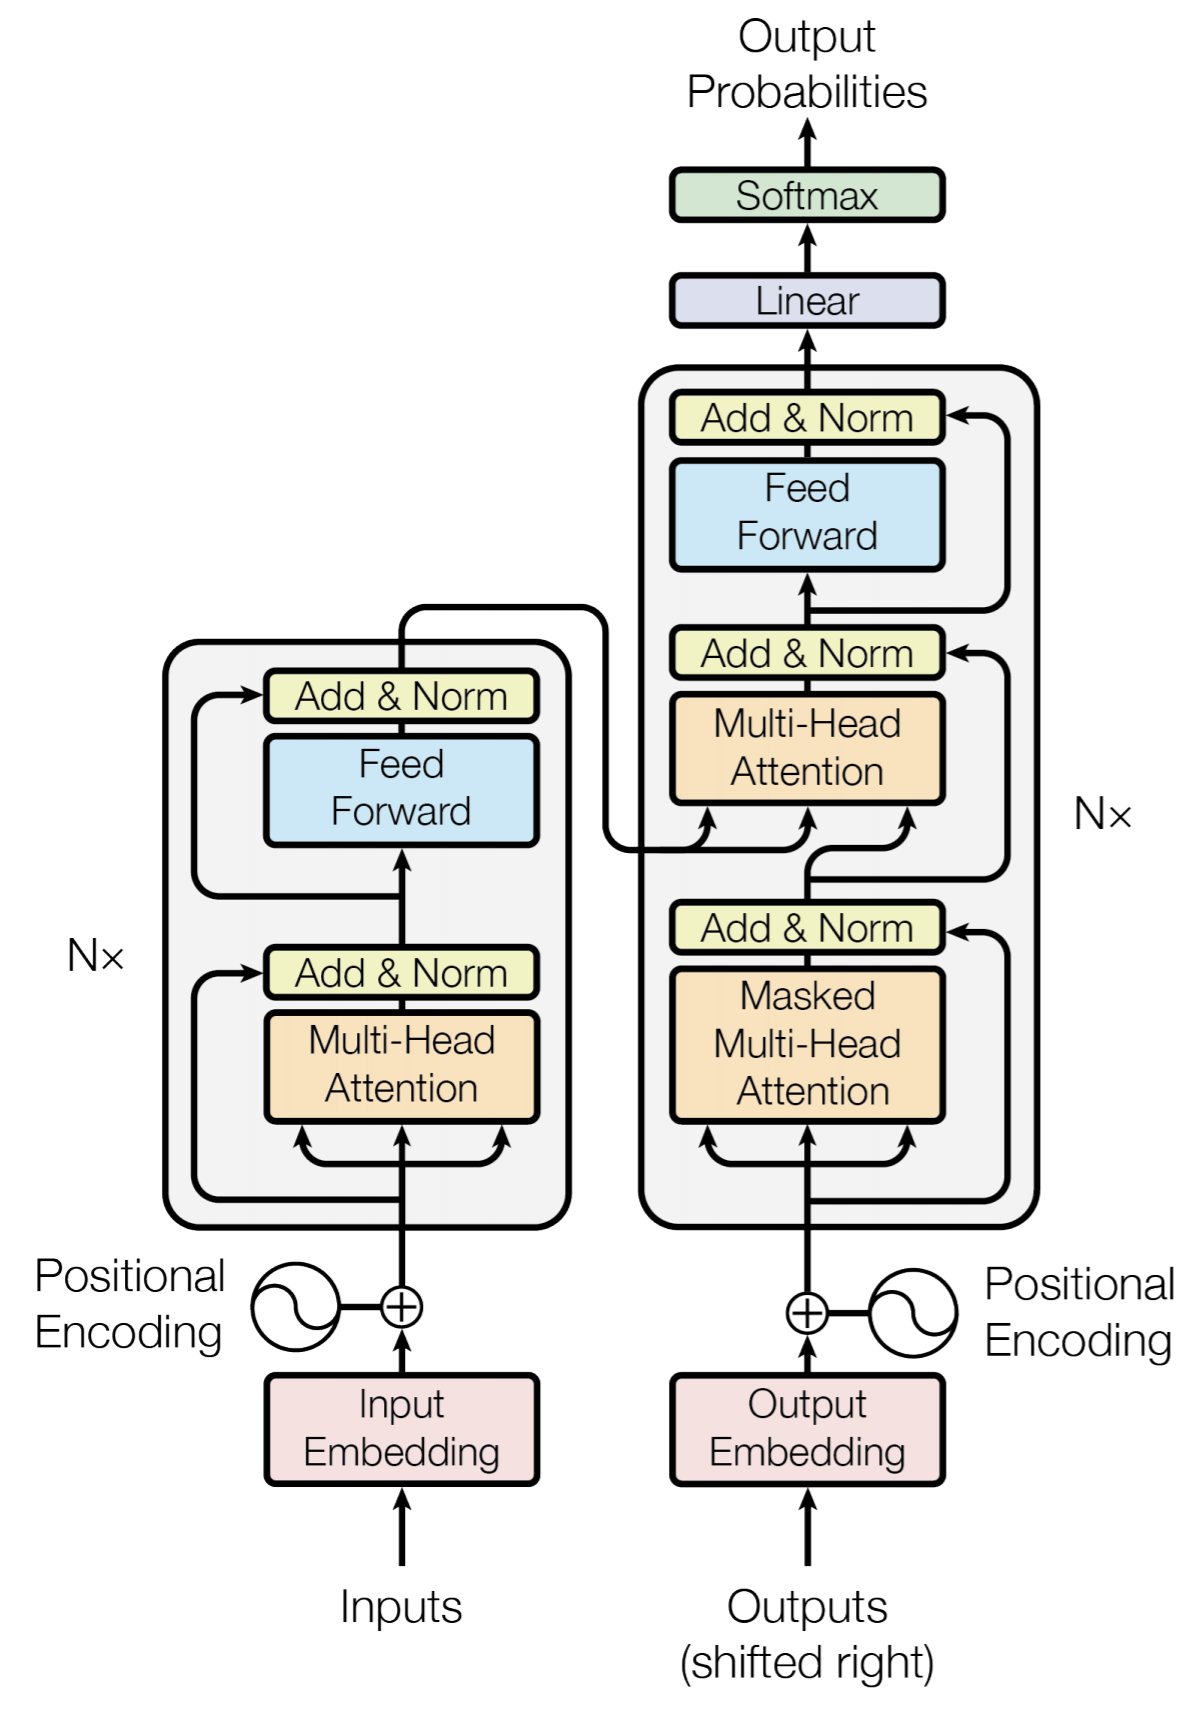
\includegraphics[width=60mm]{imgs/transformer_model.png}
  \caption{Transformer Model.}
  \label{fig:Transformer}
\end{figure}

\subsection*{Word Vectors}

We used the following two vector models to train our own word embeddings:

\begin{itemize}
  \item Word2Vec
  \item FastText
\end{itemize}

The main difference between the two models is that, where Word2Vec treats all the words individually, FastText treats each word as a sum of n-grams. FastText is essentially and extension of Word2Vec. This implicitly allows for splitting into subwords, as well as retrieving out-of-vocabulary(OOV) words by splitting it up into n-grams.

In addition to the two different kinds of models, both CBOW and skip-gram were applied for both models, resulting into four different word embeddings per language. The other hyperparameters can be found in table \ref{tb:embedding_params}.

\begin{table}[H]
  \begin{center}
    \begin{tabular}{p{4cm}|p{4cm}}
        \textbf{Parameter}& \textbf{Word2Vec/FastTex}\\
        \hline
        Minimum Word Count      & 20        \\
        Window Size             & 5         \\
        Embedding Size          & 100       \\
        Initial Learning Rate   & 0.03      \\
        Minimum Learning Rate   & 0.0007    \\
    \end{tabular}
    \caption{Word2Vec and FastText parameters}
    \label{tb:embedding_params}
  \end{center}
\end{table}

\subsection*{Evaluation Metrics}

\paragraph{BLUE} The BiLingual Evaluation Understudy algorithm \cite{Papineni2002} counts N-gram overlaps between the machine translation output and its' reference translations. This metric is position independent, so it doesn't matter where matches happened. The more matches, the better the translation is. BLEU also takes into account the length of the candidate translation, penalizing shorter translations in order to hopefully assign a better score to a more complete translation. We use N-grams up to size 4, with smoothing for those whose count ends up being 0, so as to avoid a zero final score.

\begin{equation}
BLEU = min \Big( 1, \frac{\text{output\_length}}{\text{reference\_length}}
\Big)
\big(
\prod_{i=1}^{N} precision_{i}
\big)^{\frac{1}{N}}
\end{equation}

\section*{Experiments}

For conducting experiments with models and data described above, we used the combinations of languages, vector models and translation models that are stated in Table \ref{tb:models}. The description of architectures are provided in paragraphs below. Also, numerical parameters of models are stated in Table \ref{tb:params}.

\paragraph{RNN} As it was mentioned above, Recurrent Model consists of Encoder and Decoder parts. Encoder takes the input words of the source language, transfers them to vector space and passes these vectors to GRU cell to calculate the vector representation of input sentence. Then Decoder starts translating to the target language. Decoder consists of Embedding part, GRU cell and Linear output layer with LogSoftmax activation. GRU cell takes the vector representation of input sentence as the initial hidden state. Linear layer predicts the vector, that shows the next word, so it has the length of the size of target vocabulary. Decoder works recursively starting from the start-of-sentence token. Decoder predicts the next word using the predicted word from previous iteration during validation time. During training we can use the word of target sequence. In order to avoid overfitting and improve performance, we can use the same technique as for validation (feeding predicted words) with some probability. This approach is called Teacher Forcing. For training the Negative Log Likelihood Loss is minimized. Encoder and Decoder are trained separately with separate Adam optimizers with standard PyTorch parameters.

\paragraph{Transformer} The architecture of Transformer implies the Encoder-Decoder architecture. Idea is the same as with RNN - source language input sentence is encoded and then used by Decoder recursively to translate it in target sentence. Encoder consists of several blocks. Each block has Embedding layer followed by layers shown on Figure \ref{fig:Transformer}. We also use Positional Encoding described in the original paper. FeedForward part is a perceptron with stated below layers. The same description may be applied to the Decoder architecture. The LogSoftmax non-linearity is applied in the output layer. For training the Negative Log Likelihood Loss is minimized. Encoder and Decoder are trained separately with separate Naom optimizers, which showed efficiency for Transformer's learning. This kind of optimizer firstly increase the learning rate and then gradually decrease it.

The layers of perceptron in Transformer's Encoder and Decoder:
\begin{itemize}
    \item Linear layer with Hidden Size
    \item Dropout with DropOut probability
    \item ReLU activation
    \item Linear layer
\end{itemize}


\begin{table}[h!]
  \begin{center}
    \begin{tabular}{p{4cm}|p{2cm}|p{2cm}}
        & \textbf{RNN} & \textbf{Transformer}\\
        \hline
        Batch size (in training)      & 16     & 16     \\
        Hidden Size                   & 256    & 256    \\
        Embedding Size                & 100    & 100    \\
        Teacher Forcing Prob.         & 0.5    &        \\
        DropOut Prob.                 &        & 0.1    \\
        Num. Blocks                   &        & 3      \\
        Num. Attention Heads          &        & 10     \\
    \end{tabular}
    \caption{Translation models parameters.}
    \label{tb:params}
  \end{center}
\end{table}


\paragraph{Vector Models} Training of word embeddings is done using the Python Gensim library \cite{rehurek_lrec}, which has built-in models for both Word2Vec and FastText. Because we already try out two different models, the main hyperparameter we play with is skip-gram vs. continuous bag-of-words.

Because of the corpus size, training is done in consequent batches, that need to be loaded into memory for each batch. We load in a maximum of five million lines at the time. Added to this, we \textbf{sample} our batches randomly each time. This means that in one loop over the data, we might pick some lines double, as well as skipping some others. However, as we do many loops over the entire dataset, we still train on the entire corpus. The main reason for this implementation is to simplify the application of batch learning. The resulting word embeddings are shown in the appendix, figures \ref{fig:embedding_en}, \ref{fig:embedding_nl} and \ref{fig:embedding_ru}.

Our experiment compared the performance of various kinds of word embeddings at the task of machine translation. It includes the complete process, from training the vectors to training the models. It was done over two language pairs due to time constraints, but the scripts we developed can seamlessly be used on new language pairs.


\section*{Results}

As it was mentioned above, we used the BLEU score to evaluate the performance of our translation models. In order to understand the results better, we calculated average, median, maximum and minimum scores for validation sentences. These scores are provided in Table \ref{tb:models}. The training was performed on GPUs, but due to the amount of data, the process has been taking much time. Training the for one epoch has been taking approximately 15 hours and 19 hours for Transformer and RNN respectively. For models that used FastText for embeddings it was even slower. So, due to the time restrictions of the project, we couldn't spend weeks for training and we stated the number of iterations done for each model in Table \ref{tb:models}.

It can be seen from the BLUE scores, that the best model for Russian language is RNN with skip-gram W2V and for Dutch one - Transformer with CBOW FastText.

In general the BLEU scores achieved by our models are not very high. There are several main reasons behind that:
\begin{itemize}
    \item The training data is relatively dirty and even after the preprocessing described above we faced many examples with obviously wrong or wrongly aligned  and shortened translation. For instance:
    \begin{itemize}
        \item \textbf{English sentence:} Since you're here already, do you want to take a test? Do you have any thoughts on being a producer?
        \selectlanguage{russian}
        \item \textbf{Russian sentence:} не хочешь ли принять участие в кастинге на должность продюсера ?
    \end{itemize}
    \item Due to the time restrictions, the time of training was small, as it is shown in Table \ref{tb:models}.
    \item There is a lot of space for improving the processing of unknown tokens, which could highly influence the scores.
\end{itemize}

However, looking on the examples, we can surely conclude, that even with all mentioned restrictions, our models learnt the mappings between words across languages and Language Models, what allow them to provide quite good translations, especially for simple and relatively short sentences. The examples below is taken from the test set. The first one is a long sentence translated by Transformer with CBOW embedding. The model didn't find several words, but it caught the grammatical structure very well:

\textbf{English:} All right, let me call my family and tell them they're gonna have to take care of themselves for a bit.

\selectlanguage{russian}
\textbf{Russian translation (our model):} хорошо , дай мне <UNK> семьи и сказать им , что они должны <UNK> их.

\selectlanguage{russian}
\textbf{Reference translation:} хорошо , позвоню своей семье и скажу им , что они должны сами немного позаботиться о себе.

\selectlanguage{russian}
\textbf{Google translation:} Хорошо, позвольте мне позвонить моей семье и сказать им, что им придется немного позаботиться о себе.\\

The second pair of examples are short sentences with good translation. The only confused part in the first one is the name, which model changed for another name. And our translation of the second sentence is synonym to the reference one. This is illustrated nicely if we compare the BLEU score to the length off the input sentence:

\selectlanguage{english}
\begin{figure}
    \centering
    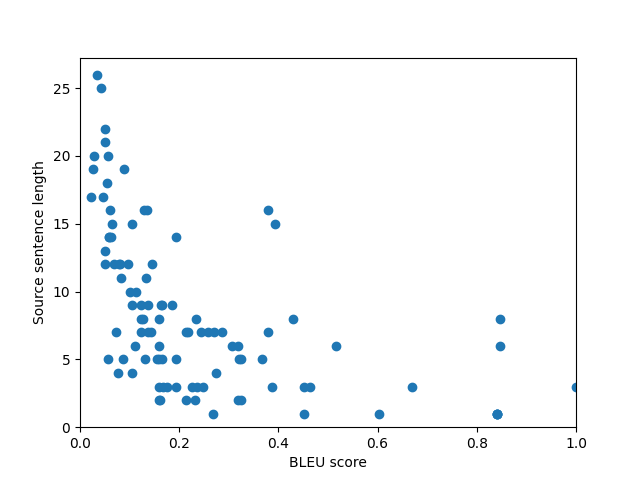
\includegraphics[width=\textwidth]{imgs/rnn_en_ru_VM_w2v_en_d100_sg_st_VM_w2v_ru_d100_sg_st_length_score.png}
    \caption{Correlation of input sentence length and BLUE score}
    \label{fig:scores_lens}
\end{figure}

The plot was done for 100 samples, and it shows that longer sentences do tend to have lower translation scores. The causes of this are discussed further in the conclusion.


\textbf{English:} Sharon is not my mother.

\selectlanguage{russian}
\textbf{Russian translation (our model):} эстер не моя мать.

\selectlanguage{russian}
\textbf{Reference translation:} шэрон - не моя мать.\\

\textbf{English:} I was only...

\selectlanguage{russian}
\textbf{Russian translation (our model):} я был только...

\selectlanguage{russian}
\textbf{Reference translation:} я лишь...\\

Also, there are several sentences of our composition of different levels, that are provided in Table \ref{tb:translation_tr_ru}. The translation to Russian is done with Recurrent model with W2V and to Dutch - with Transformer with FastText. These examples are listed to show the strengths and weaknesses of our models. It can be seen that in several cases Dutch translation is better - besides other reasons, we connect this fact to the grammatical complexity of Russian language over Dutch.

\selectlanguage{russian}
\begin{sidewaystable}
  \begin{center}
    \begin{tabular}{p{3.5cm}|p{3.5cm}|p{3.5cm}|p{3.5cm}|p{3.5cm}}
        \textbf{English sentence} & \textbf{Translation RU\newline (our model)} & \textbf{Translation RU\newline (Google)} & \textbf{Translation NL\newline (Google)} & \textbf{Translation NL\newline (Google)}\\
        \hline
        I want to buy a cat. 
        & я хочу купить кошку. 
        & Я хочу купить кошку. 
        & ik wil een kat kopen. 
        & Ik wil een kat kopen.\\
        \hline
        I want him to be a doctor. 
        & я хочу, чтобы он был врач. 
        & Я хочу, чтобы он был доктором. 
        & ik wil dat hij een dokter is. 
        & Ik wil dat hij dokter wordt.\\
        \hline
        I wish this trip would never end. 
        & не хочу, чтобы это путешествие. 
        & Я бы хотел, чтобы эта поездка никогда не закончилась. 
        & ik wens dat deze reis nooit eindigt. 
        & Ik wou dat deze reis nooit zou eindigen.\\
        \hline
        Whoever sells the most wins a trip to Disneyland. 
        & кто-то, на на... 
        & Тот, кто продает больше всего, выигрывает поездку в Диснейленд. 
        & wie de meeste wint een reis naar brooklyn. 
        & Wie het meeste verkoopt, wint een reis naar Disneyland.\\
        \hline
        Jordanian law does not impose any gender-based conditions upon passport applicants. 
        & <UNK> <UNK> не <UNK> <UNK> <UNK> <UNK> <UNK>.. 
        & Закон Иордании не устанавливает каких-либо гендерных условий для заявителей на паспорт. 
        & <UNK> heeft geen keuze van de <UNK>. 
        & De Jordaanse wet legt paspoortaanvragers geen op geslacht gebaseerde voorwaarden op.\\
        \hline
        Let's consider this thought as an offer. 
        & считай, что это предложение. 
        & Давайте рассмотрим эту мысль как предложение. 
        & laten we dit eens eens eens eens eens eens eens zien. 
        & Laten we deze gedachte beschouwen als een aanbod.\\
        \hline
        Do you want to talk about it? 
        & хочешь поговорить об этом? 
        & ты хочешь поговорить об этом? 
        & wil je erover praten? 
        & Wil je erover praten?\\
        \hline
        How long have you been in Paris? 
        & сколько ты долго в париже? 
        & Как долго вы были в Париже? 
        & hoelang ben je in parijs geweest? 
        & Hoe lang ben je al in Parijs?\\
    \end{tabular}
    \caption{Translation examples for Transformer with Russian language.}
    \label{tb:translation_tr_ru}
  \end{center}
\end{sidewaystable}

\begin{sidewaystable}
  \begin{center}
    \begin{tabular}{p{2cm}|p{2cm}|p{2cm}|p{2cm}|p{2.5cm}|p{1.5cm}|p{1.5cm}|p{1.5cm}|p{1.5cm}}
        \textbf{Translation Model} & \textbf{Vector Model} & \textbf{Language (source)} & \textbf{Language (target)} & \textbf{Training Time} & \textbf{BLEU (avg.)} & \textbf{BLEU (med.)} & \textbf{BLEU (min)} & \textbf{BLEU (max)}\\
        \hline
        RNN         & W2V\newline (skip-gram)      & English & Dutch   & 2 epochs\newline 260 000 batches & 0.2413 & 0.1454 & 0.0126 & 1.0000\\
        RNN         & W2V\newline (CBOW)           & English & Dutch   & 1 epoch\newline 415 000 batches  & 0.2385 & 0.1454 & 0.0127 & 1.0000\\
        Transformer & W2V\newline (skip-gram)      & English & Dutch   & 3 epochs\newline 375 700 batches & 0.2546 & 0.1726 & 0.0174 & 1.0000\\
        Transformer & W2V\newline (CBOW)           & English & Dutch   & 2 epochs\newline 40 500 batches  & 0.2597 & 0.1787 & 0.0003 & 1.0000\\
        RNN         & FastText\newline (skip-gram) & English & Dutch   & 0 epochs\newline 663 000 batches & 0.2183 & 0.1432 & 0.0101 & 1.0000\\
        RNN         & FastText\newline (CBOW)      & English & Dutch   & 0 epochs\newline 262 000 batches & 0.2290 & 0.1426 & 0.0093 & 1.0000\\
        Transformer & FastText\newline (skip-gram) & English & Dutch   & 5 epochs                         & 0.2504 & 0.1749 & 0.0129 & 1.0000\\
        Transformer & FastText\newline (CBOW)      & English & Dutch   & 2 epochs\newline 854 600 batches & \textbf{0.2827} & 0.1928 & 0.0248 & 1.0000\\
        RNN         & W2V\newline (skip-gram)      & English & Russian & 2 epochs\newline 42 000 batches  & \textbf{0.2860} & 0.1923 & 0.0164 & 1.0000\\
        RNN         & W2V\newline (CBOW)           & English & Russian & 1 epoch\newline 800 000 batches  & 0.2776 & 0.1797 & 0.0128 & 1.0000\\
        Transformer & W2V\newline (skip-gram)      & English & Russian & 3 epochs\newline 30 600 batches  & 0.2647 & 0.1797 & 0.0062 & 1.0000\\
        Transformer & W2V\newline (CBOW)           & English & Russian & 2 epochs\newline 632 200 batches & 0.2447 & 0.1749 & 0.0257 & 1.0000\\
        RNN         & FastText\newline (skip-gram) & English & Russian & 2 epochs\newline 625 000 batches & 0.2777 & 0.1797 & 0.0146 & 1.0000\\
        RNN         & FastText\newline (CBOW)      & English & Russian & 0 epochs\newline 330 000 batches & 0.2650 & 0.1739 & 0.0149 & 1.0000\\
        Transformer & FastText\newline (skip-gram) & English & Russian & 6 epochs\newline 402 700 batches & 0.2474 & 0.1634 & 0.0228 & 1.0000\\
        Transformer & FastText\newline (CBOW)      & English & Russian & 6 epochs\newline 244 800 batches & 0.2404 & 0.1638 & 0.0172 & 1.0000\\
    \end{tabular}
    \caption{Experiments setup (models, languages) and results.}
    \label{tb:models}
  \end{center}
\end{sidewaystable}



\section*{Conclusions}

The ultimate goal of the project, machine translation done from the ground up out of single-language and aligned corpora, has been achieved with moderate success. Translation is not done word for word, and also takes into account other words in the sentence, but seems to struggle with longer inputs, as seen on \ref{fig:scores_lens}. Presumably this is due to the training time, the sizes of our models, and would have been much better if we could have made models with more layers, bigger hidden sizes, more attention heads etc. 

There are several possible ways for improving our work. Firstly, several techniques can allow us to squeeze the size of output SoftMax layer to decrease the size of both models. This layer is the performance bottleneck, so we estimate the possible improvements to be substantial. The models could also be trained for longer, as we had to ration our resources to train all 16 models to a reasonable degree without using too many Aalto resources.

Because of the architecture of the models, which use the indices of the words in the vocabulary for inputs and outputs, one feature of FastText isn't used - it doesn't have OOV words, but represents them through their N-grams. In our implementation, those words are replaced with an unknown token. The reason is connected to our current realization of models architecture on PyTorch and time restrictions of the project.

Additional models could also be tested, the most obvious of which would be RNNs with the attention mechanism built in. Another important approach that should be tried, especially in context of Transformer models, is BERT model, which is a pre-trained Encoder of Transformer for specific tasks. Since the project specification requires exploration the words vector representation, we left the BERT outside the scope of this project.

The BLEU score is also one possible point of improvement, due to its' inherent flaws. Given that we only have one reference per test sample this would render all synonyms as incorrect translations for example. Since our dataset is also noisy and includes dialog with words from the spoken language used to improve the flow of the sentence (words such as uhm, ah and so on), it can be translated in many different ways, thus potentially impacting the end result. A cleaner test set would probably allow more accurate scores using BLEU, and using other metrics might give an even more accurate picture.

\newpage

\selectlanguage{english}
\printbibliography

\newpage

\section*{Division of labor}

\begin{itemize}
  \item Andrey Sukhobok
    \begin{itemize}
        \item Training translation models
        \item Developing Transformer model
        \item Writing python code
        \item Writing report
    \end{itemize}
  \item Kosta Stanojević
    \begin{itemize}
        \item Training translation models
        \item Developing Recurrent model
        \item Writing python code
        \item Writing report
    \end{itemize}
  \item Rob Verbeek
    \begin{itemize}
        \item Training vector models
        \item Data and model's utilities preparation
        \item Writing python code
        \item Writing report
    \end{itemize}
\end{itemize}

\section*{Appendix}

\begin{itemize}
  \item GitHub with code: \url{https://github.com/RobZelluf/NLP_vector_project}
  \item Data: \url{http://opus.nlpl.eu/OpenSubtitles-v2018.php}
\end{itemize}

\newpage

\selectlanguage{english}
\begin{figure}
    \centering
    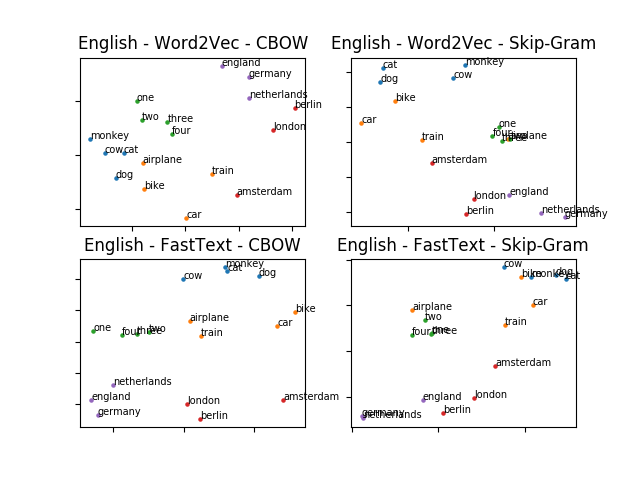
\includegraphics[width=\textwidth]{imgs/embedding_en.png}
    \caption{Example of relative position of words in Vector Model (English).}
    \label{fig:embedding_en}
\end{figure}

\selectlanguage{english}
\begin{figure}
    \centering
    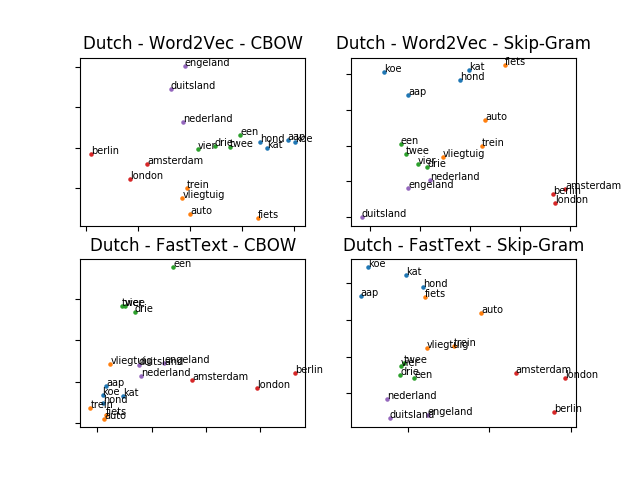
\includegraphics[width=\textwidth]{imgs/embedding_nl.png}
    \caption{Example of relative position of words in Vector Model (Dutch).}
    \label{fig:embedding_nl}
\end{figure}

\selectlanguage{english}
\begin{figure}
    \centering
    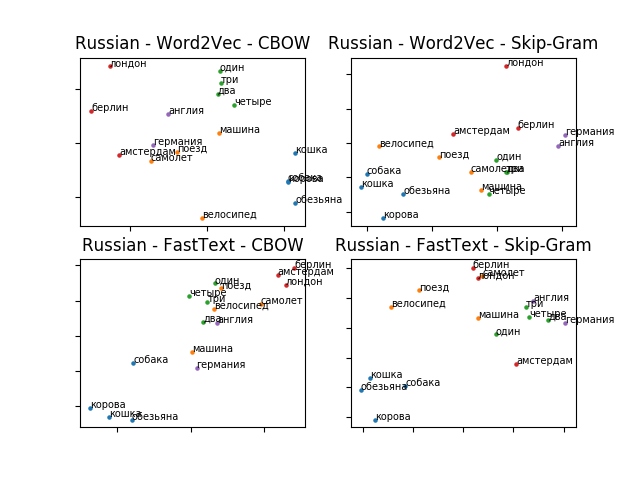
\includegraphics[width=\textwidth]{imgs/embedding_ru.png}
    \caption{Example of relative position of words in Vector Model (Russian).}
    \label{fig:embedding_ru}
\end{figure}

\end{document}
